\chapter{Wstęp}
\vspace{-30pt}
\section{Wprowadzenie do tematu }
Chcąc nauczyć się grać utwór muzyczny na instrumencie klawiszowym, najpierw trzeba nabyć umiejętność czytania nut oraz znaleźć zapis nutowy danej piosenki. Można również wyświetlić piosenkę w postaci graficznie przedstawionych wskazówek, które klawisze należy naciskać i jak długo (tzw. synthesii), aby zagrać dany utwór, niemniej jednak wymaga to od nas znalezienia gotowej animacji, bądź piosenki w formacie muzycznym midi, który rzadko występuje oraz program, który ten format przekonwertuje i wyświetli. Dużo łatwiej uzyskać plik muzyczny wav lub mp3. Dzięki postępom w dziedzinie analizy sygnałów audio możliwe stało się mapowanie dźwięków z plików mp3 na sekwencje nut w formacie midi. Ten proces konwersji, wykorzystujący zaawansowane techniki przetwarzania sygnałów, otwiera drzwi do nowych metod edukacyjnych, umożliwiając naukę gry na instrumentach muzycznych w interaktywny i atrakcyjny sposób.
\section{Cel pracy inżynierskiej}
Głównym celem niniejszej pracy inżynierskiej jest stworzenie programu w postaci gry muzycznej zintegrowanej z elektronicznym instrumentem klawiszowym, gdzie następuje przedstawienie w postaci graficznej wyznaczonych uprzednio tonów i porównywanie do sygnału odbieranego z keyboardu oraz naliczanie punktów za poprawne odwzorowywanie sekwencji klawiszy.
Dodatkowym wyzwaniem jest również opracowanie sposobu konwersji plików muzycznych z formatu mp3 do formatu midi poprzez przeanalizowanie sygnału audio z wykorzystaniem transformaty Fouriera i analityczne wyznaczenie częstotliwości z powstałego widma.
\newpage
\section{Struktura i zakres pracy}
W dalszej części pracy zostały szczegółowo omówione teoretyczne podstawy syntezy dźwięku oraz analizy sygnałów audio. Następnie została przedstawiona metodyka obejmująca proces konwersji plików mp3 do formatu midi. Kolejny rozdział zawiera szczegółowy opis implementacji gry umożliwiającej wizualizację wygenerowanej synthesii interaktywnej z keyboardem użytkownika, co pozwala na uzyskiwanie punktów za poprawne powtarzanie wyświetlonej sekwencji klawiszy.

\begin{figure}[h]
  \centering
  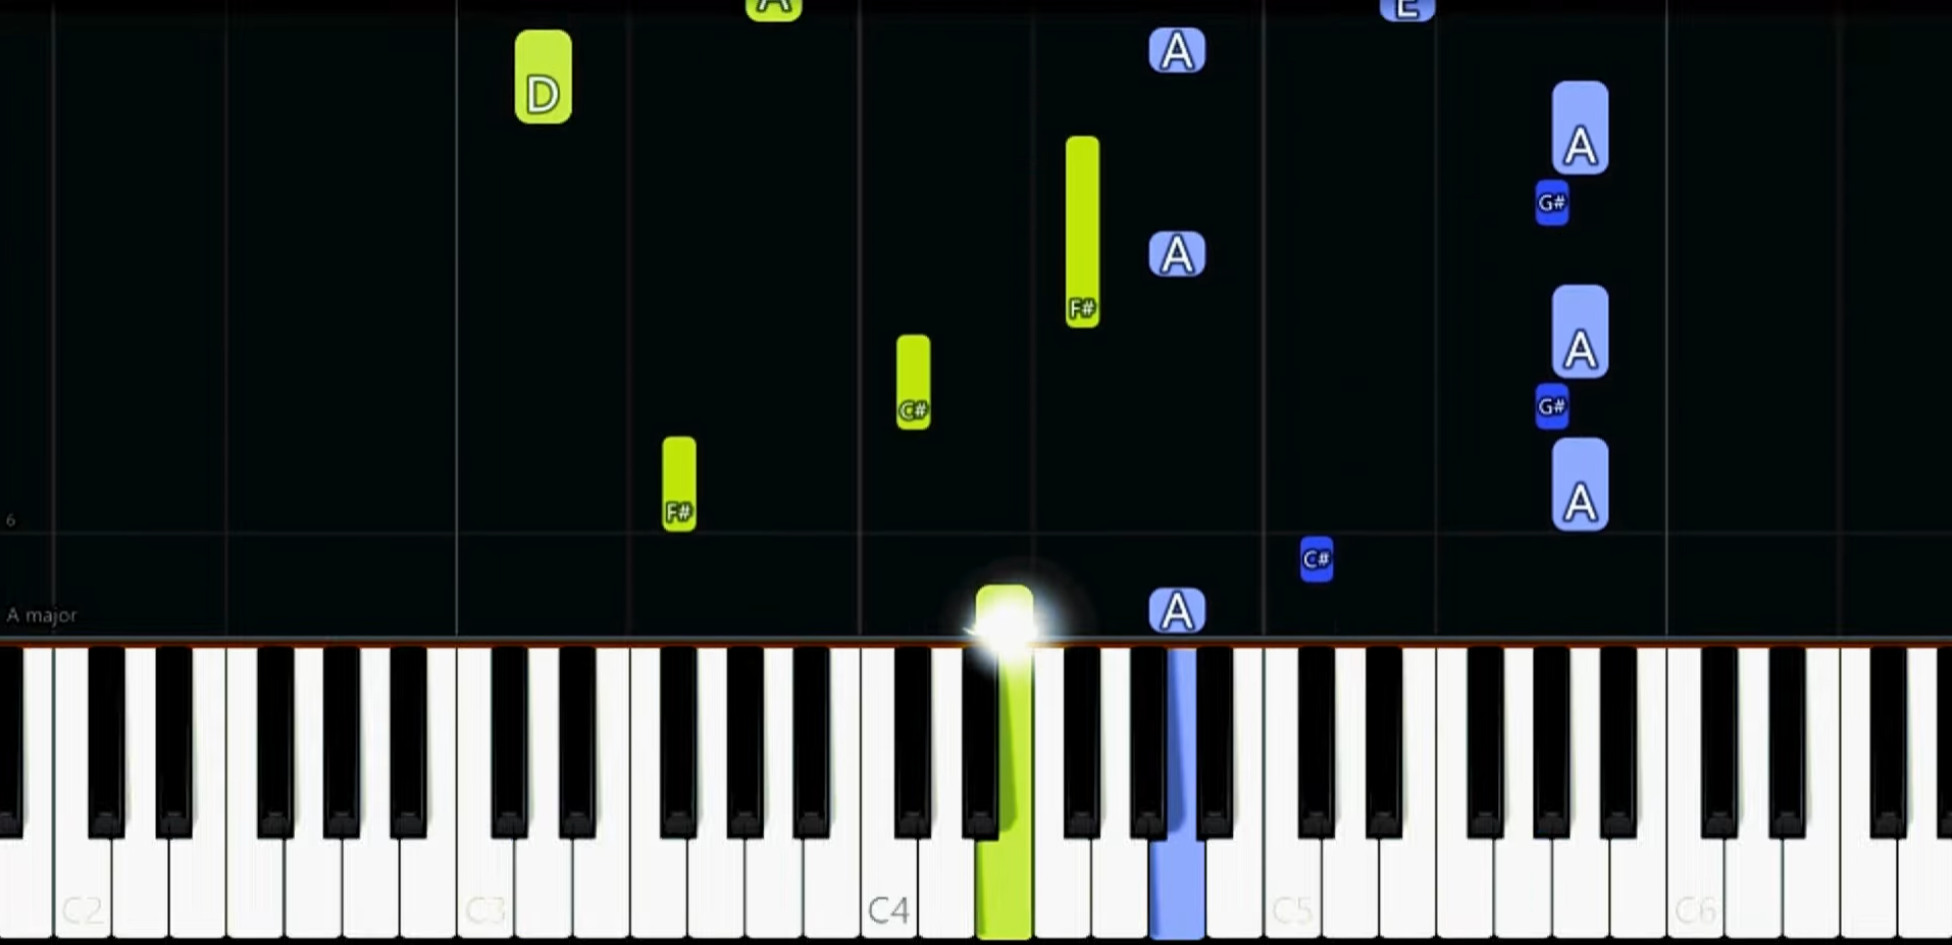
\includegraphics[width=1\textwidth]{img/1/image.png}
  \caption{Przykładowa synthesia przedstawiająca piosenkę Yiruma - "River Flows In You"\cite{synthesia}}
\end{figure}

Dalsza część pracy poświęcona będzie testowaniu projektu i analizie uzyskanych wyników, rozważań nad osiągniętymi rezultatami oraz perspektywom rozwoju projektu w kontekście możliwych usprawnień i dalszych badań. Niniejsza praca stanowi wkład w rozwój technologii przetwarzania sygnałów audio oraz otwiera nowe możliwości w zakresie interaktywnej edukacji muzycznej i kreatywnej ekspresji dźwiękowej. Eksploracja tych zaawansowanych technik konwersji dźwięku ma na celu stworzenie narzędzia, które może znaleźć zastosowanie w edukacji oraz rozrywce.
\newpage
\section{Wykorzystane narzędzia}

Implementacja gry muzycznej z użyciem instrumentu klawiszowego wymaga bardzo elastycznego i nieograniczającego środowiska oraz wielu narzędzi, które zapewnią wiele możliwości na jakże obszernym polu, które obejmuje projekt. Środowisku, które sprawdzi się w analizie sygnałów dźwiękowych, pozwalające również na przetwarzanie dużej ilości danych w krótkim czasie, aby program był użytkowy. Idealnie do powyższej problematyki wpasowuje się język programowania {Python} \cite{python}, często wybierany w projektach związanych z przetwarzaniem wszelakich sygnałów ze względu na elastyczność, prostotę i bogactwo w dostępności bibliotek pomocnych w obliczeniach takich jak {NumPy} \cite{numpy}, do pracy z dźwiękiem jak przykładowo {LibROSA} \cite{librosa}, czy do wizualizacji danych takich jak {Matplotlib} \cite{matplotlib}.

Bardzo ważnym elementem jest biblioteka {Pygame} \cite{pygame}, która pomaga nie tylko w tworzeniu projektu w postaci gry, ale również sprawdza się jako pomoc przy znalezieniu podłączonego instrumentu muzycznego i odebraniu z niego danych. Zazwyczaj komputery osobiste nie posiadają wejścia MIDI, ale użycie interfejsu audio MIDI USB \cite{roland_um_one} marki Roland pozwala przetworzyć sygnał pochodzący z instrumentów, takich jak np. keyboard CASIO \cite{casio_ctk496}.

Jednak aby można było wykorzystać instrument w testowaniu projektu, niezbędna jest możliwość przetworzenia sygnału midi na plik muzyczny oraz manipulowania nim w kolejnych etapach, w czym nieocenione były narzędzia {FluidSynth} \cite{fluidsynth} oraz {FFmpeg} \cite{ffmpeg} dające szerokie spektrum możliwości.

Aby dokładnie przeprowadzić analizę sygnału ścieżki audio niezbędnym narzędziem jest transformata Fouriera \cite{fourier_transform_visual}\cite{dsp_understanding}, która pozwala spojrzeć na ten sam sygnał w całkowicie inny sposób.

Ostatnią czynnością pozostało zamknięcie wszystkich elementów w jedną całość, zachowując pełną funkcjonalność, jednakże nie odstając szatą graficzną. Pozwoliło na to użycie {pygame-menu} \cite{pygame_menu} oraz {Tkinter} \cite{tkinter} dzięki czemu gotowy program nie tylko jest efektywny, ale również efektowny.
